\usetikzlibrary{calc}
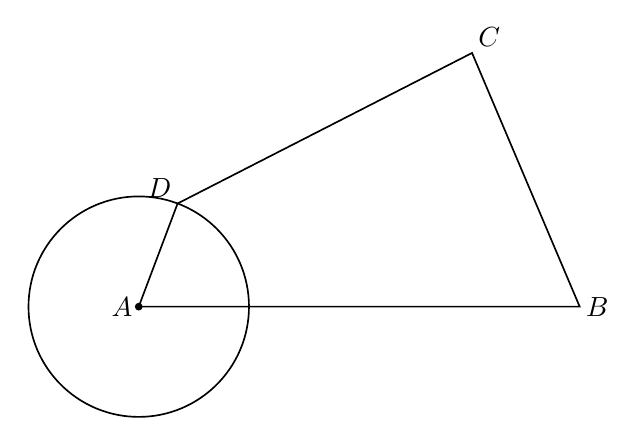
\begin{tikzpicture}[x=1cm,y=1cm,line width=.6pt,font=\normalsize]
\coordinate (A) at (0,0);
\coordinate (B) at (5.6,0);
\coordinate (C) at (4.2332,3.2221);
\coordinate (D) at (0.4937,1.3101);
\draw (A)--(D)--(C)--(B)--cycle;
\draw (A) circle[radius=1.4cm];
\node[left=2pt,inner sep=0pt] at (A) {$A$};
\node[right=2pt,inner sep=0pt] at (B) {$B$};
\node[above right=2pt,inner sep=0pt] at (C) {$C$};
\node[above left=2pt,inner sep=0pt] at (D) {$D$};

% Explicit named circle-center points, painted after all region fills.
\fill (A) circle[radius=1.4pt];
\end{tikzpicture}
